
%%%%%%%%%%%%%%%%%%%%%%%%%%%%%%%%%%%%%%%%%%%%%%%%%%%%%%%%%%%%%%%%%
%% All content of these notes are part of a textbook that is being %%printed and is planned to be published in 2025/26. 
%% All these notes belong to, created by, and copyrighted for 
%% Ghassan AlRegib and Mohit Prabhushankar
%% Georgia Tech, 2024-2025
%%%%%%%%%%%%%%%%%%%%%%%%%%%%%%%%%%%%%%%%%%%%%%%%%%%%%%%%%%%%%%%%%



%%%%%PLEASE CONSIDER CORRECTIONS AT PLACES INDICATED%%%%%%%%
\documentclass{article}
%%%%%Packages Used, add more if necessary%%%%
\usepackage{amsmath,amsfonts,amssymb,graphicx,fullpage,float}
\setlength{\topmargin}{-0.6 in}
\setlength{\textheight}{8.5 in}
\setlength{\headsep}{0.75 in}
\usepackage{mdframed}
\usepackage{multicol}
\usepackage{microtype}
\usepackage{hyperref}
\usepackage{natbib}
\bibliographystyle{plain}

%%%%% NO NEED TO EDIT THIS PREAMBLE %%%%%%%%
%%% PREAMBLE %%%
\newcounter{lecnum}
\renewcommand{\thepage}{\thelecnum-\arabic{page}}
\renewcommand{\thesection}{\thelecnum.\arabic{section}}
\renewcommand{\theequation}{\thelecnum.\arabic{equation}}
\renewcommand{\thefigure}{\thelecnum.\arabic{figure}}
\renewcommand{\thetable}{\thelecnum.\arabic{table}}
\newcommand{\lecture}[4]{
   \pagestyle{myheadings}
   \thispagestyle{plain}
   \newpage
   \setcounter{lecnum}{#1}
   \setcounter{page}{1}
   \noindent
   \begin{center}
   \framebox{
      \vbox{\vspace{2mm}
      
      \hbox to 6.28in { 
      {\bf ECE 4252/6252 (FunML) Fundamentals of Machine Learning \hfill 2021--2028} }
      
      \vspace{2mm}
      \hbox to 6.28in { 
      {Courses developed by Professor Ghassan AlRegib 
      (\href{https://alregib.ece.gatech.edu/}{alregib.ece.gatech.edu}) 
      \hfill For inquiries: \href{mailto:alregib@gatech.edu}{alregib@gatech.edu}} }
      
      \vspace{3mm}
      \hbox to 6.28in { {\Large \hfill Lecture #1: #2 \hfill} }
      
      \vspace{2mm}
      \hbox to 6.28in { {\it Co-Instructors: #3 \hfill #4} }
      
      \vspace{2mm}}
   }
   \end{center}

   % -------- PEOPLE OUTSIDE BOX --------
   \vspace{2mm}
   \noindent{\bf Contributors:} Dr. Ahmad Mustafa, Dr. Motaz Alfarraj, Dr. Ashraf Alattar, Dr. Chen Zhou

   \vspace{1mm}
   \noindent{\bf Teaching Assistants} with remarkable contributions include: Kuo-Wei Lai, Wuyang Du, Shiva Mahato, Michael Zhou, Ninghan Zhong

   \markboth{Lecture #1: #2}{Lecture #1: #2}

      \vspace{3mm}
   \noindent {\bf Disclaimer}: 
   {All content of these notes are part of this course at Georgia Tech. Any re-use or distribution is not permitted without pre-approved permission. All these notes belong to, created by, and copyrighted for Ghassan AlRegib and Mohit Prabhushankar, Georgia Tech, 2021--2028.}

      \vspace{2mm}
    \noindent {\bf License}: 
    {These lecture notes are licensed under the 
    \href{https://creativecommons.org/licenses/by-nc-sa/4.0/}{Creative Commons Attribution-NonCommercial-ShareAlike 4.0 International License}.}


   \vspace{2mm}
   \noindent {\bf Errata}: 
   {\it Please submit any errata you find using the following form: 
   \href{https://forms.office.com/r/fbg9dMWPgY}{Errata Form for FunML Textbook} 
   or visit: \url{https://forms.office.com/r/fbg9dMWPgY}}

   \vspace*{4mm}
}
% \renewcommand{\cite}[1]{[#1]}
% \def\beginrefs{\begin{list}
%         {[\arabic{equation}]}{\usecounter{equation}
%          \setlength{\leftmargin}{2.0truecm}\setlength{\labelsep}{0.4truecm}%
%          \setlength{\labelwidth}{1.6truecm}}}
% \def\endrefs{\end{list}}
% \def\bibentry#1{\item[\hbox{[#1]}]}

\newcommand{\challenge}[2]{\noindent \textbf{(Challenge Problem)} \emph{#1}: #2 }

\newcommand{\exercise}[1]{\noindent \textbf{(Exercise)} #1 }

\newcommand{\fig}[3]{
			\vspace{#2}
			\begin{center}
			Figure \thelecnum.#1:~#3
			\end{center}
	}
%%% END_OF_PREAMBLE %%%


	
%%%%You may add more \newtheorem if necessary%%%%%%
\newtheorem{theorem}{Theorem}[lecnum]
\newtheorem{lemma}[theorem]{Lemma}
\newtheorem{proposition}[theorem]{Proposition}
\newtheorem{claim}[theorem]{Claim}
\newtheorem{corollary}[theorem]{Corollary}
\newtheorem{definition}[theorem]{Definition}
\newenvironment{proof}{{\bf Proof:}}{\hfill\rule{2mm}{2mm}}


\newcommand{\dom}{\mathrm{dom}}
\begin{document}

%%%%%CHANGE HERE%%%%%%%
%%%%%\section{title of the section} similarly with the rest \section{} or \subsection{} or \subsubsection{} etc


%%%%%CHANGE HERE%%%%%%%%%
%%%%%\lecture{the ordinal number of the lecture}{lecture title}{Jacob Abernethy}{scriber's name}%%%%%%%%
\lecture{1}{Introduction to Machine Learning}{Ghassan AlRegib and Mohit Prabhushankar}{}%%{Fahd Aly, Nikolaos Komianos}

\section{Lecture Objectives}

This lecture introduces the fundamental concepts that form the foundation of machine learning. We begin by distinguishing artificial intelligence, machine learning, and deep learning, and by discussing how machines acquire and use knowledge compared to humans. We then present the main machine learning paradigms, including supervised, unsupervised, and reinforcement learning, along with common machine learning tasks such as regression, classification, clustering, and dimensionality reduction. The lecture also provides a high-level overview of deep learning and its growing impact. Finally, we review the essential mathematical foundations required for the course, including core concepts from linear algebra and probability theory that will be used throughout subsequent lectures.

\section{Artificial Intelligence}

There is no universally accepted definition of artificial intelligence (AI), partly because natural intelligence itself is not fully understood or formally defined. In general, AI refers to a system's ability to correctly interpret external data, learn from that data, and use those learnings to achieve specific goals and tasks through flexible adaptation.

Artificial intelligence, sometimes called machine intelligence or computational intelligence, describes intelligence demonstrated by machines, in contrast to the natural intelligence displayed by humans. AI is often used to describe systems that mimic cognitive functions typically associated with the human mind, such as learning, reasoning, and problem solving. Early AI systems were primarily rule-based, meaning that all rules and exceptions had to be explicitly programmed by humans.

Despite advances in automation, humans still play a critical role in the development, supervision, and improvement of AI systems. Human expertise is often required to design models, interpret results, and ensure that AI systems operate reliably and ethically.

\subsection{Humans vs AI}

AI-driven applications typically excel in speed of execution, computational accuracy, and the ability to perform repetitive or large-scale tasks without fatigue. These systems are particularly effective in tedious and monotonous jobs such as large-scale data analysis, automated inspection, and pattern detection across massive datasets. In contrast, human intelligence is characterized by adaptive learning, reasoning from limited data, creativity, and the ability to transfer knowledge across different domains. Unlike most AI systems, humans do not always rely on large amounts of pre-labeled data to learn new concepts \cite{springboard_ai}.

Despite the impressive capabilities of modern AI systems, humans still play a central role in defining problems, curating data, interpreting results, and ensuring responsible use of these technologies. AI systems are tools that augment human decision making rather than completely replace it.

One of the true challenges of artificial intelligence is solving tasks that are easy for humans to perform but difficult to formalize mathematically. For example, humans can recognize faces, understand sarcasm in language, or navigate unfamiliar environments with little effort, yet these tasks remain challenging for AI systems because they require complex perception, context understanding, and generalization abilities.

\section{Knowledge}

Knowledge can generally be categorized into three main types: explicit knowledge, implicit knowledge, and tacit knowledge. Understanding these distinctions is important in machine learning because different types of knowledge require different approaches for representation and learning.

Explicit knowledge refers to knowledge that is easy to articulate, document, and share with others. This type of knowledge can be written down in textbooks, manuals, or databases and is often structured in a way that allows it to be easily communicated. For example, a factual statement such as ``The capital of the State of Georgia is Atlanta'' represents explicit knowledge because it can be clearly expressed and transferred between individuals or systems.

Implicit knowledge refers to the practical application of explicit knowledge. It often involves skills or procedures that can be learned through instruction and practice. Unlike explicit knowledge, implicit knowledge is demonstrated through action rather than simply stated as facts. For example, knowing how to operate a photocopier or apply a known procedure in a new setting represents implicit knowledge, as it involves applying previously learned information to accomplish a task.

Tacit knowledge refers to knowledge gained through personal experience that is often difficult to express formally or transfer through written or verbal communication. This type of knowledge typically develops through practice, observation, and intuition. Examples include skills such as swimming, reading social cues, speaking fluently in a language, or recognizing faces. Tacit knowledge is particularly challenging for artificial intelligence systems because it is difficult to fully formalize or encode into explicit rules.

\section{Machine Learning}

Machine learning (ML) is a subset of artificial intelligence that focuses on developing algorithms that can learn patterns from data and improve their performance over time without being explicitly programmed for every possible scenario. Instead of relying on manually written rules, machine learning systems build mathematical models using sample data, commonly referred to as training data, to make predictions or decisions.

Traditional rule-based AI systems require engineers to explicitly define all rules and exceptions. While effective for well-defined problems, these systems often fail when dealing with complex environments where rules are difficult to specify. Machine learning addresses this limitation by allowing systems to automatically discover patterns and relationships directly from data. This makes ML particularly useful in applications where the underlying structure of the problem is unknown or too complex to model manually.

Machine learning is considered superior to purely rule-based approaches in many real-world scenarios because it can adapt to new data, generalize to unseen situations, and improve performance as more data becomes available. Examples of successful machine learning applications include machine translation, recommender systems, fraud detection, speech recognition, and medical diagnosis.

At a high level, a machine learning system typically follows three main steps:
\begin{itemize}
    \item \textbf{Training:} The model learns patterns from labeled or unlabeled data.
    \item \textbf{Validation:} The model is evaluated and tuned to improve performance.
    \item \textbf{Testing:} The trained model is applied to new unseen data.
\end{itemize}

Machine learning has enabled major advances across many fields, particularly in areas involving large amounts of data. Some of the most important application domains are described below.

\subsection{Recommendation Systems}

Recommendation systems are machine learning systems designed to suggest relevant items to users based on their preferences, behavior, or similarities to other users. These systems are widely used in online platforms to personalize user experiences and increase engagement.

For example, streaming platforms such as Netflix recommend movies based on viewing history, e-commerce platforms such as Amazon recommend products based on browsing behavior, and music platforms such as Spotify recommend songs based on listening patterns. These systems often rely on techniques such as collaborative filtering, content-based filtering, or hybrid approaches that combine both methods.

The key challenge in recommendation systems is predicting user preferences from incomplete and noisy data. Machine learning models address this by identifying hidden patterns in user interactions and learning similarities between users or items.

\subsection{Computer Vision}

Computer vision is a field of machine learning focused on enabling machines to interpret and understand visual information such as images and videos. This area has seen significant advances due to deep learning, particularly through convolutional neural networks (CNNs).

Common computer vision tasks include image classification, object detection, image segmentation, and facial recognition. For example, autonomous vehicles rely on computer vision to detect pedestrians and traffic signs, medical imaging systems use computer vision to detect tumors, and security systems use facial recognition for identity verification.

One of the main challenges in computer vision is dealing with variations in lighting, viewpoint, noise, and occlusion. Machine learning models address these challenges by learning robust feature representations directly from large image datasets.

\subsection{Natural Language Processing}

Natural language processing (NLP) focuses on enabling machines to understand, interpret, and generate human language. Because human language is highly ambiguous and context dependent, NLP remains one of the most challenging areas of artificial intelligence.

Examples of NLP applications include machine translation, chatbots, sentiment analysis, speech recognition, and text summarization. Modern NLP systems often rely on deep learning architectures such as transformers, which power large language models like GPT.

The main challenge in NLP is enabling machines to capture meaning, context, and relationships between words. Machine learning models address this by learning statistical representations of language from large text corpora, allowing systems to recognize patterns in syntax, semantics, and context.

Together, these application areas demonstrate the broad impact of machine learning across technology, science, and society. As computational resources and data availability continue to grow, machine learning is expected to play an increasingly important role in solving complex real-world problems.

\section{Paradigms of Machine Learning}

Machine learning algorithms can be broadly categorized based on the type of data available during training and how the learning process is structured. The three primary paradigms are supervised learning, unsupervised learning, and reinforcement learning. Each paradigm differs in how information is provided to the model and what objective the model attempts to optimize.

\subsection{Supervised Learning}

Supervised learning is the most common machine learning paradigm and involves training a model using labeled data. In this setting, each training example consists of an input along with a corresponding correct output, often called a label. The goal of supervised learning is to learn a mapping from inputs to outputs so that the model can accurately predict labels for new, unseen data.

For example, in an image classification task, a dataset may contain images of cats labeled as 0 and images of dogs labeled as 1. The model learns patterns that distinguish these categories and uses those patterns to classify new images. Other examples include predicting housing prices from property features (regression) or identifying whether an email is spam or not (classification).

Supervised learning problems are typically divided into two major categories: regression, where the goal is to predict continuous values, and classification, where the goal is to predict discrete categories.

\subsection{Unsupervised Learning}

Unsupervised learning involves training models on data that does not include labels. Instead of learning a mapping between inputs and outputs, the goal is to discover hidden structure or patterns within the data itself. This often involves grouping similar data points together or identifying meaningful low-dimensional representations of the data.

For example, given a collection of audio recordings without speaker labels, an unsupervised learning algorithm might group recordings according to similarities in voice characteristics. Similarly, unsupervised learning can be used in customer segmentation, anomaly detection, and dimensionality reduction.

Common unsupervised learning techniques include clustering algorithms such as k-means and hierarchical clustering, as well as dimensionality reduction methods such as principal component analysis (PCA).

\subsection{Reinforcement Learning}

Reinforcement learning differs from supervised and unsupervised learning in that the model learns by interacting with an environment rather than from a fixed dataset. In this paradigm, an agent takes actions within an environment and receives feedback in the form of rewards or penalties. The goal of the agent is to learn a strategy, called a policy, that maximizes the total cumulative reward over time.

For example, in a game such as Tetris, an agent may receive a positive reward for clearing rows and a negative reward for creating blocked spaces. By repeatedly interacting with the environment and observing the consequences of its actions, the agent gradually learns which actions lead to better long-term outcomes.

Reinforcement learning has been successfully applied in robotics, game playing, recommendation systems, and autonomous systems. One of the key challenges in reinforcement learning is balancing exploration (trying new actions to gain information) with exploitation (choosing actions known to produce good results).

\section{Tasks in Machine Learning}

Machine learning problems can be categorized in two complementary ways. Learning paradigms describe how models learn from data (for example supervised, unsupervised, or reinforcement learning), while machine learning tasks describe what the model is expected to predict or discover. In this section, we focus on the most common machine learning tasks.

Machine learning tasks are typically categorized based on the type of output a model is expected to produce during testing. These tasks define the objective of the learning process and determine how model performance is evaluated. Some of the most common machine learning tasks include regression, classification, clustering, and dimensionality reduction.

\subsection{Regression}

Regression refers to predicting a continuous numerical value based on one or more input variables. In regression problems, the output variable typically represents a measurable quantity such as price, temperature, probability, or risk score. The goal of regression is to learn the relationship between input variables (independent variables) and the output variable (dependent variable) so that accurate predictions can be made on unseen data.

For example, a regression model may be used to predict housing prices based on features such as square footage, number of bedrooms, and location. Other examples include predicting stock prices, estimating medical risk scores, forecasting energy consumption, or predicting traffic flow. In each case, the model attempts to learn a functional relationship between inputs and outputs.

Common regression models include linear regression, polynomial regression, decision trees, and neural networks. Later in this course, we will study regression as one of the fundamental problems that motivates many machine learning algorithms.

\subsection{Classification}

Classification refers to predicting which category or class a new observation belongs to. Unlike regression, where outputs are continuous, classification produces discrete outputs representing class membership. The goal is to learn decision boundaries that separate different categories based on the input features.

For example, classification models can be used to determine whether an email is spam or not, whether a medical image contains a tumor, whether a handwritten digit corresponds to a particular number, or whether a financial transaction is fraudulent. Classification problems may be binary (two classes) or multiclass (more than two classes).

Common classification algorithms include logistic regression, decision trees, support vector machines, nearest neighbor methods, and neural networks. Many modern artificial intelligence applications rely heavily on classification models, particularly in computer vision and natural language processing.

\subsection{Clustering}

Clustering is an unsupervised learning task that involves dividing data into groups, called clusters, such that data points within the same group are more similar to each other than to those in other groups. Unlike classification, clustering does not require labeled data and instead attempts to discover natural structure within the dataset.

For example, clustering may be used to segment customers based on purchasing behavior, group similar documents together, organize images by visual similarity, or identify patterns in biological data. The main challenge in clustering is defining what it means for data points to be similar and determining the appropriate number of clusters.

Common clustering methods include k-means clustering, hierarchical clustering, Gaussian mixture models, and density-based clustering methods. Clustering is often used as an exploratory tool to better understand datasets before applying supervised learning methods.

\subsection{Dimensionality Reduction}

Dimensionality reduction involves reducing the number of features or variables in a dataset while preserving as much important information as possible. This is often necessary because high-dimensional data can be computationally expensive to process and may contain redundant, irrelevant, or noisy information.

For example, an image consisting of thousands of pixels may be represented using a smaller set of informative features without significantly affecting performance. Dimensionality reduction is commonly used for data visualization, noise reduction, feature extraction, and improving computational efficiency. It also helps mitigate the curse of dimensionality, which refers to the challenges that arise when working with very high-dimensional datasets.

Common dimensionality reduction techniques include principal component analysis (PCA), singular value decomposition (SVD), manifold learning methods, and neural network–based approaches such as autoencoders.

These tasks form the foundation of many machine learning applications, and many real-world systems combine multiple tasks together. For example, a computer vision system may first reduce dimensionality to extract meaningful features, then cluster similar patterns, and finally perform classification to recognize objects.

Importantly, these tasks often align with the learning paradigms introduced earlier. For example, regression and classification are typically supervised learning tasks because they require labeled data, while clustering and dimensionality reduction are usually unsupervised learning tasks. Reinforcement learning, in contrast, focuses on sequential decision-making problems where an agent learns through interaction with an environment rather than through static prediction tasks.


\section{Deep Learning}

Deep learning is a subfield of machine learning that focuses on models capable of learning hierarchical representations directly from data. These models learn multiple levels of abstraction, allowing machines to build complex concepts from simpler ones. For example, in image recognition tasks, early layers of a deep neural network may learn to detect edges, later layers may learn shapes, and deeper layers may learn object-level representations.

One of the major advantages of deep learning is its ability to perform end-to-end learning. Traditional machine learning methods often rely on manually designed features, which require significant domain expertise and engineering effort. In contrast, deep learning models automatically learn useful feature representations directly from raw data, reducing the need for manual feature engineering and often improving performance.

Although the first artificial neural network models were proposed in the 1950s, deep learning only became widely successful in the last two decades. This progress has been driven by three main factors: the availability of large datasets, significant increases in computational power (particularly through GPUs and specialized hardware), and improvements in training algorithms.

Modern deep learning models have grown significantly in size and capability. For example, large language models such as GPT-based systems contain billions or even trillions of parameters and are capable of performing tasks such as text generation, reasoning, translation, and question answering. The increasing real-world impact of deep learning has led to major investments from academia and industry, accelerating research and deployment across fields such as healthcare, autonomous systems, robotics, and scientific discovery.

Because deep learning models rely heavily on mathematical optimization, linear algebra, and probability theory, understanding these mathematical foundations is essential for studying modern machine learning methods.

\section{AI vs ML vs DL}

Artificial intelligence (AI), machine learning (ML), and deep learning (DL) are closely related fields that are often confused. Artificial intelligence is the broadest concept and refers to systems designed to perform tasks that typically require human intelligence. Machine learning is a subset of AI that focuses on algorithms that learn patterns from data rather than relying solely on explicitly programmed rules. Deep learning is a further subset of machine learning that focuses on neural networks with multiple layers capable of learning hierarchical representations.

\begin{figure}[H]
\centering
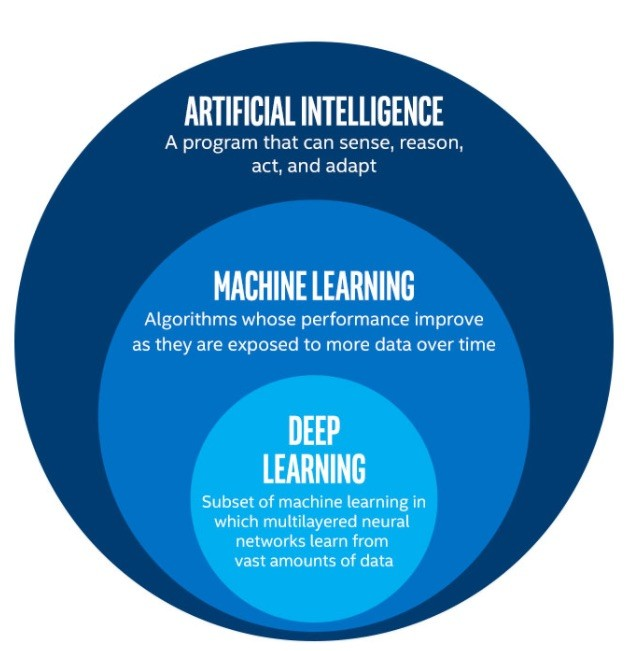
\includegraphics[width=0.55\textwidth]{img/lecture1/AI_ML_DL_circles.jpeg}
\caption{Figure 1.1: Relationship between artificial intelligence, machine learning, and deep learning. Deep learning is a subset of machine learning, which itself is a subset of artificial intelligence.}
\label{fig:ai_ml_dl}
\end{figure}

Figure~\ref{fig:ai_ml_dl} illustrates the relationship between these three areas. Machine learning represents a subset of artificial intelligence that focuses specifically on data-driven learning methods, while deep learning represents a subset of machine learning that uses multi-layer neural networks to automatically learn feature representations.

Compared to deep learning, traditional machine learning methods often rely more heavily on manually designed features, a process known as feature engineering. Designing these features can require significant domain knowledge and time. Deep learning reduces this need by automatically learning useful representations directly from raw data, allowing models to develop complex concepts from simpler patterns.

For example, in a traditional computer vision system, engineers might manually design features such as edge detectors or texture descriptors. In contrast, a deep learning model can automatically learn these features during training, often achieving better performance when sufficient data is available.

Understanding the relationship between AI, ML, and DL helps clarify the scope of this course. While artificial intelligence is a broad discipline, this course primarily focuses on the mathematical foundations of machine learning, including the principles that also support modern deep learning systems.



\section{Review of Linear Algebra}

Linear algebra forms one of the most important mathematical foundations of machine learning. Most machine learning models represent data, parameters, and predictions using vectors and matrices, and many learning algorithms rely heavily on matrix operations and linear transformations. In this section, we review the key linear algebra concepts that will be used throughout the course.

\subsection{Basic objects}

Machine learning models operate on several fundamental mathematical objects. The simplest of these is a scalar, which is a single numerical value such as $x \in \R$. Scalars are often used to represent individual measurements, parameters, or outputs.

A vector is an ordered collection of numbers, typically represented as a column vector $\mathbf{x} \in \R^{n\times 1}$. Vectors are commonly used to represent data points, feature sets, or parameter collections in machine learning. For example, a data sample with $n$ features can be represented as a vector containing those feature values.

A matrix is a two-dimensional array of numbers, denoted $A \in \R^{m\times n}$, where $m$ represents the number of rows and $n$ represents the number of columns. Matrices are often used to represent datasets, where rows correspond to samples and columns correspond to features. Matrices also represent transformations applied to vectors, such as weight matrices in neural networks.

A tensor is a higher-order generalization of vectors and matrices. Tensors are multi-dimensional arrays used to store structured data such as images, videos, or batches of features. For example, a color image may be represented as a three-dimensional tensor (height, width, color channels), while a batch of images may be represented as a four-dimensional tensor.

\subsection{Why linear algebra matters in ML}

Linear algebra provides the language used to describe most machine learning models. Data points are typically represented as vectors, model parameters are represented as matrices, and predictions are often computed using matrix operations.

For example, consider a linear model that predicts outputs from input features. A data sample may be represented as a feature vector $\mathbf{x}_i \in \R^d$. A linear model may then compute a prediction using:

\[
\mathbf{y}_i = W^\top \mathbf{x}_i + \mathbf{b},
\]

where $W$ is a weight matrix and $\mathbf{b}$ is a bias vector. This type of linear transformation appears throughout machine learning, including regression, classification, and neural networks.

Because modern machine learning relies heavily on these representations, understanding linear algebra is essential for understanding how models process data and learn patterns.

\subsection{Essential operations}

Several fundamental linear algebra operations appear repeatedly in machine learning algorithms. One important operation is the inner product (or dot product), defined as:

\[
\langle \mathbf{x}, \mathbf{y} \rangle = \mathbf{x}^\top \mathbf{y} = \sum_i x_i y_i.
\]

This operation measures similarity between vectors and appears frequently in similarity measures, projections, and optimization objectives.

Another important operation is matrix-vector multiplication, written as:

\[
A\mathbf{x} = \mathbf{b}.
\]

This represents applying a linear transformation to a vector and is the core operation used in linear models and neural networks.

Matrix multiplication is also fundamental:

\[
C = AB, \qquad A \in \R^{m\times n},\; B \in \R^{n\times p},\; C \in \R^{m\times p}.
\]

This operation allows multiple linear transformations to be composed together and is heavily used in deep learning architectures.

The Hadamard product, written as:

\[
(A \odot B)_{ij} = A_{ij} B_{ij},
\]

refers to elementwise multiplication and is commonly used in neural network operations and attention mechanisms.

Finally, the transpose operation:

\[
(A^\top)_{ij} = A_{ji}
\]

swaps the rows and columns of a matrix and appears frequently in optimization and matrix decompositions.

\subsection{Identity and inverse}

The identity matrix $I_n \in \R^{n\times n}$ is a special matrix that leaves vectors unchanged when multiplied:

\[
I_n \mathbf{x} = \mathbf{x}.
\]

This matrix plays a role similar to the number 1 in multiplication.

If a matrix $A$ is invertible, then there exists another matrix $A^{-1}$ such that:

\[
A^{-1}A = I_n.
\]

Matrix inverses appear in many machine learning algorithms, particularly in closed-form solutions such as least squares regression. However, not all matrices are invertible, and in practice numerical methods are often preferred over direct inversion.

\subsection{Norms}

Norms are functions that measure the magnitude or size of vectors and matrices. They are commonly used in machine learning to measure error, regularization penalties, and distances between data points.

Some common vector norms include:

\begin{align*}
\|\mathbf{x}\|_1 &= \sum_i |x_i|, \\
\|\mathbf{x}\|_2 &= \left(\sum_i x_i^2\right)^{1/2}, \\
\|\mathbf{x}\|_p &= \left(\sum_i |x_i|^p\right)^{1/p}.
\end{align*}

The $\ell_1$ norm is often used in sparse modeling, while the $\ell_2$ norm appears frequently in optimization and regularization.

For matrices, a common norm is the Frobenius norm:

\[
\|A\|_F = \left(\sum_{i,j} A_{ij}^2\right)^{1/2} = \sqrt{\Tr(AA^\top)}.
\]

This norm measures the overall magnitude of a matrix and is often used in optimization objectives.

\subsection{Eigenvalues and eigenvectors}

Eigenvalues and eigenvectors describe important structural properties of matrices. For a matrix $A$, an eigenvector is a vector whose direction remains unchanged when multiplied by the matrix, while the eigenvalue describes how much that vector is scaled.

If a matrix is diagonalizable, it can be written as:

\[
A = V\,\mathrm{diag}(\lambda)\,V^{-1},
\]

where the columns of $V$ are eigenvectors and $\lambda$ contains the eigenvalues.

Eigenvalues and eigenvectors are fundamental in many machine learning methods, including principal component analysis (PCA), spectral clustering, and stability analysis of learning algorithms.

\subsection{Singular value decomposition (SVD)}

The singular value decomposition (SVD) is one of the most important matrix factorizations in machine learning. For any matrix $A \in \R^{m\times n}$, SVD allows us to write:

\[
A = UDV^\top,
\]

where:
\begin{itemize}
    \item $U$ contains left singular vectors,
    \item $D$ contains singular values,
    \item $V$ contains right singular vectors.
\end{itemize}

SVD provides a way to understand the structure of a matrix and is widely used in data analysis, dimensionality reduction, and numerical optimization.

\subsubsection*{Why SVD appears in ML}

SVD plays an important role in dimensionality reduction. If $X \in \R^{N\times P}$ is a data matrix, we can approximate it using only the largest singular values and their corresponding vectors. A rank-$q$ approximation keeps only the dominant singular directions, reducing feature dimension from $P$ to $q$ while preserving most of the important information.

This idea forms the mathematical basis of principal component analysis (PCA), which is widely used for feature extraction and visualization.

\subsection{Moore--Penrose pseudoinverse}

In many machine learning problems, matrices are not square or not invertible. In these cases, we use the Moore--Penrose pseudoinverse, which generalizes the concept of matrix inversion.

If $A = UDV^\top$, then the pseudoinverse is defined as:

\[
A^{\dagger} = VD^{-1}U^\top,
\]

where inversion is applied only to nonzero singular values.

The pseudoinverse is particularly important in machine learning because it provides closed-form solutions for least squares problems and appears in many optimization methods.

\section{Review of Probability Theory}

Probability theory provides the mathematical framework for reasoning about uncertainty. Since machine learning models must make predictions from incomplete or noisy data, probability plays a central role in modeling uncertainty, estimating parameters, and evaluating predictions. Many machine learning algorithms, including regression, classification, and deep learning, can be interpreted through a probabilistic lens.

In this section, we review the core probability concepts that will be used throughout the course.

\subsection{Foundational objects}

Probability theory begins with three fundamental components. The first is the sample space, denoted $\Omega$, which represents the set of all possible outcomes of a random experiment. For example, if we flip a coin, the sample space is:

\[
\Omega = \{\text{Heads}, \text{Tails}\}.
\]

The second component is the event space $\mathcal{F}$, which consists of subsets of the sample space. Each subset represents an event of interest. For example, the event of obtaining heads corresponds to the subset $\{\text{Heads}\}$.

The third component is the probability measure $P$, which assigns probabilities to events. The probability measure defines how likely each event is and must obey certain mathematical rules.

Together, $(\Omega, \mathcal{F}, P)$ define a probability space.

\subsection{Axioms of probability}

Probability is governed by three basic axioms. For any event $A \in \mathcal{F}$, the probability must satisfy:

\begin{align*}
0 &\le P(A) \le 1, \\
P(\Omega) &= 1.
\end{align*}

The first axiom states that probabilities must lie between zero and one. The second states that the probability of all possible outcomes occurring must equal one.

A third important rule concerns mutually exclusive events. If events $A_1, A_2, \dots$ cannot occur simultaneously, then:

\[
P\!\left(\bigcup_i A_i\right) = \sum_i P(A_i).
\]

This rule allows probabilities of disjoint outcomes to be added together.

\subsection{Useful rules}

Several important rules follow directly from the probability axioms. For example, if event $A$ is contained within event $B$, then:

\[
A \subseteq B \implies P(A) \le P(B).
\]

This reflects the intuitive idea that a more restrictive event cannot be more probable than a broader one.

Another important rule is the complement rule:

\[
P(\Omega \setminus A) = 1 - P(A),
\]

which states that the probability of an event not occurring equals one minus the probability that it does occur.

The inclusion–exclusion rule gives the probability of two events occurring:

\[
P(A \cup B) = P(A) + P(B) - P(A \cap B).
\]

Conditional probability is also fundamental:

\[
P(A \mid B) = \frac{P(A \cap B)}{P(B)}.
\]

This quantity measures how likely event $A$ is given that event $B$ has already occurred. Conditional probability forms the basis of Bayesian inference and many probabilistic machine learning models.

Two events are said to be independent if:

\[
P(A \cap B) = P(A)P(B).
\]

Independence plays an important role in simplifying probabilistic models and appears frequently in assumptions made by machine learning algorithms.

\subsection{Random variables}

A random variable is a function that maps outcomes from the sample space to real numbers:

\[
X : \Omega \to \R.
\]

Random variables allow us to convert outcomes into numerical quantities that can be analyzed mathematically.

Random variables are typically categorized as either discrete or continuous. A discrete random variable takes values from a finite or countable set, such as the outcome of rolling a die. A continuous random variable takes values from a continuous range, such as measurements of height or temperature.

Random variables are central to machine learning because they allow us to model uncertain quantities such as labels, predictions, and noise.

\subsection{PMF, CDF, and PDF}

The behavior of a random variable is described by its probability distribution.

For a discrete random variable $X$, the probability mass function (PMF) is defined as:

\[
p_X(x) = P(X=x).
\]

This function assigns a probability to each possible value and must satisfy:

\[
0 \le p_X(x) \le 1, \qquad \sum_x p_X(x)=1.
\]

The cumulative distribution function (CDF) is defined as:

\[
F_X(x) = P(X \le x).
\]

The CDF applies to both discrete and continuous variables and describes the probability that the random variable is less than or equal to a given value.

For continuous random variables, probabilities are described using the probability density function (PDF):

\[
f_X(x) = \frac{d}{dx}F_X(x).
\]

The PDF must satisfy:

\[
\int_{-\infty}^{\infty} f_X(x)\,dx = 1.
\]

Unlike discrete probabilities, continuous densities do not directly give probabilities at a single point. Instead, probabilities are computed over intervals.

\subsection{Joint distributions and the chain rule}

Machine learning often involves multiple random variables. Their relationships are described using joint distributions.

For two random variables $X$ and $Y$, the joint distribution describes their simultaneous behavior:

\begin{align*}
p_{X,Y}(x,y) &= P(X=x, Y=y), \\
F_{X,Y}(x,y) &= P(X\le x, Y\le y).
\end{align*}

From joint distributions we can derive conditional distributions, which are heavily used in probabilistic modeling.

A key identity is the chain rule of probability:

\[
p(x_1,x_2,\dots,x_n) = p(x_1)\prod_{i=2}^n p(x_i\mid x_1,\dots,x_{i-1}).
\]

This factorization is extremely important in machine learning because it allows complex distributions to be broken into simpler conditional relationships. Many modern models, including graphical models, autoregressive models, and transformers, rely on this factorization idea.

\subsection{Expectation, variance, and covariance}

Expectation represents the average value of a random variable. For a discrete random variable:

\[
\E[X] = \sum_x x p_X(x),
\]

and for a continuous random variable:

\[
\E[X] = \int_{-\infty}^{\infty} x f_X(x)\,dx.
\]

Expectation plays a central role in machine learning because many learning objectives involve minimizing expected error.

Variance measures how spread out a random variable is around its mean:

\[
\Var(X) = \E[(X-\E[X])^2].
\]

Covariance measures how two variables vary together:

\[
\Cov(X,Y) = \E[(X-\E[X])(Y-\E[Y])].
\]

These quantities are important in machine learning because they describe uncertainty, feature relationships, and appear in methods such as PCA and Gaussian models.

\subsection{Important distributions}

Certain probability distributions appear frequently in machine learning.

\subsubsection*{Bernoulli distribution}

The Bernoulli distribution models binary outcomes such as success/failure or true/false. For a random variable $X \in \{0,1\}$ with parameter $q$:

\[
P(X=1)=q, \qquad P(X=0)=1-q.
\]

This can also be written compactly as:

\[
P(X=x)=q^x(1-q)^{1-x}, \qquad x\in\{0,1\}.
\]

Bernoulli distributions form the basis of binary classification models such as logistic regression.

\subsubsection*{Gaussian distribution}

The Gaussian (normal) distribution is one of the most important distributions in machine learning. A univariate Gaussian with mean $\mu$ and variance $\sigma^2$ has density:

\[
\mathcal{N}(x;\mu,\sigma^2) =
\frac{1}{\sqrt{2\pi\sigma^2}}
\exp\!\left(-\frac{(x-\mu)^2}{2\sigma^2}\right).
\]

Gaussian distributions are widely used because many natural processes approximately follow this distribution and because they have convenient mathematical properties.

\subsubsection*{Multivariate Gaussian distribution}

The multivariate Gaussian generalizes the Gaussian distribution to vectors. For $\mathbf{x} \in \R^n$ with mean $\boldsymbol{\mu}$ and covariance matrix $\Sigma$:

\[
\mathcal{N}(\mathbf{x};\boldsymbol{\mu},\Sigma)
=
\frac{1}{(2\pi)^{n/2}\det(\Sigma)^{1/2}}
\exp\!\left(
-\frac{1}{2}
(\mathbf{x}-\boldsymbol{\mu})^\top
\Sigma^{-1}
(\mathbf{x}-\boldsymbol{\mu})
\right).
\]

This distribution is fundamental in machine learning because it models correlated features and appears in many algorithms such as Gaussian mixture models, Bayesian inference, and Kalman filtering.

\subsection{Law of total probability}

The law of total probability allows us to decompose the probability of an event into contributions from mutually exclusive cases. Suppose $\{B_1,\dots,B_n\}$ forms a partition of the sample space (meaning the events are disjoint and cover all possibilities). Then:

\[
P(A) = \sum_{i=1}^n P(A \mid B_i)P(B_i).
\]

This rule is important because it allows us to compute probabilities by conditioning on simpler or more interpretable events.

For example, suppose we want the probability that a classifier makes an error. We may condition on the true class:

\[
P(\text{error}) =
P(\text{error} \mid y=0)P(y=0)
+
P(\text{error} \mid y=1)P(y=1).
\]

This decomposition appears frequently in machine learning when analyzing expected loss and classification error.

\subsection{Bayes rule}

Bayes rule provides a way to reverse conditional probabilities. It follows directly from the definition of conditional probability:

\[
P(A \mid B) =
\frac{P(B \mid A)P(A)}{P(B)}.
\]

Using the law of total probability, this can also be written as:

\[
P(A \mid B)
=
\frac{P(B \mid A)P(A)}
{\sum_i P(B \mid A_i)P(A_i)}.
\]

Bayes rule is fundamental in machine learning because it provides the basis for Bayesian inference and probabilistic classification.

In machine learning notation, Bayes rule is often written as:

\[
P(y \mid x)
=
\frac{P(x \mid y)P(y)}{P(x)}.
\]

This interpretation is often described as:

\[
\text{posterior} =
\frac{\text{likelihood} \times \text{prior}}
{\text{evidence}}.
\]

This formula explains how we update our belief about a label $y$ after observing data $x$. Many models such as Naive Bayes classifiers and Bayesian neural networks rely on this principle.

\subsection{Jensen's inequality}

Jensen's inequality is one of the most important mathematical tools in machine learning theory. It describes how convex functions interact with expectations.

If $f$ is a convex function and $X$ is a random variable, then:

\[
f(\E[X]) \le \E[f(X)].
\]

If $f$ is concave, the inequality reverses:

\[
f(\E[X]) \ge \E[f(X)].
\]

This result is important because many machine learning loss functions are convex, and Jensen's inequality helps us derive bounds and guarantees.

One particularly important example involves the logarithm function, which is concave:

\[
\log(\E[X]) \ge \E[\log X].
\]

This property appears frequently in machine learning, including:

\begin{itemize}
\item Log-likelihood optimization
\item Variational inference
\item EM algorithm derivations
\item KL divergence proofs
\item Risk bounds
\end{itemize}

Intuitively, Jensen's inequality tells us that applying a nonlinear transformation before averaging is not the same as applying it after averaging. This subtle difference is extremely important in statistical learning theory.

\bibliographystyle{unsrt}
\bibliography{references}

\end{document}